The different types of recommendation systems can be categorized based on from where they get the needed information to make the recommendations. (The Adaptive Web p. 379)

\begin{figure}[htb]
\centering
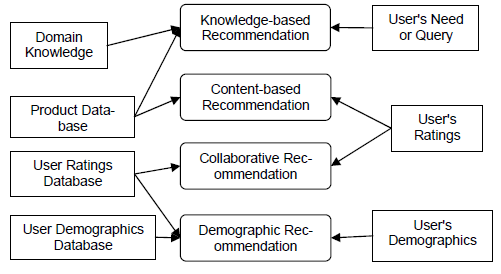
\includegraphics[width=0.8\textwidth]{Images/RecTypes.png}
\caption{Recommendation Techniques and their knowledge sources}
\label{RecTypes}
\end{figure}

The [picture] shows the four recommendation systems and what sources they use. Sometimes the sources available dictates which recommender the system must use unless a hybrid is chosen. 


\subsubsection{Collaborative Recommendations} 
\label{Collaborative} 
\relinput{Collaborative} 

\subsubsection{Content Based Recommendations} 
\label{ContentBased} 
\relinput{ContentBased}

\subsubsection{Differences}
\label{Differences} 
\relinput{Differences}

\subsubsection{Hybrid Systems} 
\label{Hybrid} 
\relinput{Hybrid}